\documentclass[12pt]{article}
\usepackage{float}
\usepackage{tabularx}
\usepackage{todonotes}
\usepackage{color, colortbl}
\usepackage{pdfpages}
\definecolor{light-gray}{gray}{0.95}
\setuptodonotes{}

% This is all the packages and settings and so on.
% It is using custom fonts that needs to be installed on the computer. If they are not present, they have to be added manually.
\usepackage[
	citestyle=ieee, 
    bibstyle=ieee,
    style=numeric-comp,
    sorting=nty, 
%     sortcites=true
    ]{biblatex}
    
% Makes the last name first in the bibliography.
\DeclareNameAlias{author}{last-first}
    
% Specify the margins
\usepackage[a4paper, margin=3cm]{geometry}

\usepackage{eso-pic}								% Packages for layout and graphics 
\usepackage{graphicx}
\usepackage{tikz}
\usepackage{setspace}
\usepackage{tocloft}		 						% Fixing a bug with page style changes for toc
\tocloftpagestyle{fancy}
\usepackage{etoc} 									%Separate tocs for appendix and the rest    
\usepackage{chngcntr}							  	% Count figures within chapters
\counterwithin{figure}{section} 
\counterwithin{table}{section}
\usepackage{booktabs}							  	% Table formatting
\usepackage{fancyhdr}								% Setting the style for header and footer.
\usepackage[hidelinks]{hyperref}					% Clickable links
\usepackage{nameref}								% References with names
\usepackage[parfill]{parskip}						% New line instead of indent for sections
\usepackage{subfig}						 			% Package for putting figures side by side
\usepackage{tcolorbox}								% Create boxes around content
\tcbset{colback=white,arc=0mm}

% Specifying fonts
\usepackage{fontspec}
\setmainfont{Georgia} 
\setsansfont{Arial}
\newfontfamily\footerfont{Georgia}

\usepackage{sectsty}
\sectionfont{\sffamily\fontsize{14}{15}}
\subsectionfont{\sffamily\fontsize{13}{15}}
\subsubsectionfont{\sffamily\fontsize{12}{15}}

% Remove the title and make sure that the text is adjusted
\usepackage{abstract}
\setlength{\absleftindent}{0mm}
\renewcommand{\abstractname}{\vspace{-\baselineskip}}
\renewcommand{\abstractnamefont}{\sffamily\fontsize{14}{15}}
\renewcommand{\abstracttextfont}{\normalfont\fontsize{12}{13}}

% Renaming and setting style of table of contents
\usepackage{tocloft}
\renewcommand*\contentsname{Contents}
\renewcommand*\cfttoctitlefont{\fontsize{16}{0}\bf\sffamily}
\renewcommand\cftsecfont{\fontsize{12}{0}\bf\sffamily}
\renewcommand\cftsecpagefont{\fontsize{12}{0}\bf\sffamily}


% Styling the header and footer
\pagestyle{fancy}
\fancyhf{}
\renewcommand{\headrulewidth}{0pt}
\fancyfoot[R]{\footerfont\thepage}

% Making the command for placing text in random locations
\newcommand\PlaceText[3]{%
\begin{tikzpicture}[remember picture,overlay]
\node[outer sep=0pt,inner sep=0pt,anchor=south west] 
  at ([xshift=#1,yshift=-#2]current page.north west) {#3};
\end{tikzpicture}%
}

% Disable hyphenation
\pretolerance=10000
\tolerance=2000 
\emergencystretch=500pt

% Custom toc for cleaner main document
\newcommand{\customtoc}{
        \etocdepthtag.toc{mtchapter}
        \etocsettagdepth{mtchapter}{subsection}
        \etocsettagdepth{mtappendix}{none}
        \newpage
        \thispagestyle{fancy}
        \tableofcontents
        % Fixing a bug where the page number would randomly fail to be right justified.
        \thispagestyle{fancy} 
        \newpage
}

% Defining files for bibliography
%\addbibresource{ref.bib}
\addbibresource{references.bib}
% Add a second bibliography file for the second author to allow
% both to update it through the mendeley integration.
% \addbibresource{ref-author-2.bib}

% Defining document information
\title{ }
\newcommand{\subtitle}{User Experience Influenced Model for Comparing Application Development Tools \newline}
\author{\textbf{Mileikowsky, Celine \newline \newline Porling, Sebastian}}

\begin{document}
\setstretch{1.4}

% The front page of the document
\makeatletter
\begin{titlepage}

\vspace*{-4.6\baselineskip}
\hspace*{-0.15\textwidth}
\includegraphics[width=0.2\paperwidth]{img/kth-logo}%
\par\vspace*{2.5\baselineskip}

\PlaceText{65mm}{12mm}{\fontsize{12}{0}\sffamily DEGREE PROJECT IN TECHNOLOGY,}
\PlaceText{65mm}{17mm}{\fontsize{12}{0}\sffamily FIRST CYCLE, 15 CREDITS}
\PlaceText{65mm}{22mm}{\fontsize{12}{0}\sffamily\itshape STOCKHOLM, SWEDEN \the\year}

~\\

\hspace*{-3cm}\begin{minipage}[b]{63.5mm}
~\\
\end{minipage}
\begin{minipage}{0.65\textwidth}
\begin{flushleft}
{\fontsize{28}{24}\bf\sffamily\@title\\}
\vspace{0.5cm}
{\fontsize{19}{17}\bf\sffamily \subtitle\\}
\vspace{0.5cm} 
{\fontsize{16}{0}\sffamily \@author}\\
\end{flushleft}

\end{minipage}


\AddToShipoutPictureBG*{%]
    \AtPageLowerLeft{%
        
\includegraphics[width=1.0\paperwidth]{img/kth-footer}%
    }%
}

\PlaceText{65mm}{280mm}{\color{white}\fontsize{12}{0}\sffamily KTH ROYAL INSTITUTE OF TECHNOLOGY }
\PlaceText{65mm}{285mm}{\color{white}\fontsize{8}{0}\sffamily ELECTRICAL ENGINEERING AND COMPUTER SCIENCE }
\end{titlepage}
\makeatother


\newpage
\pagenumbering{roman}

\newpage

%%%%%%%%%%%%%%%%%%%%%%%%%%%%%%%%%%%%
%%														 The English abstract						            		%%
%%%%%%%%%%%%%%%%%%%%%%%%%%%%%%%%%%%%
\section*{Abstract}
%%%%%%%%%%%%%%%%%%%%%%%%%%%%%%%%%%%%
There are many possible tools to develop mobile applications with. Choosing a development tool is done by considering many different factors, and the choice is currently done, in many cases, arbitrarily. For this project, a decision model is designed to ease the process of choosing a development tool.

A survey was conducted to examine how people using different smartphone platforms discover and download applications. 94 responses were collected, showing that approx. 50\% of Android-users found mobile applications by using search engines or browsers. This number was approx. 30\% for iOS-users.

A usability test was conducted to discover the differences in user experience between Progressive web applications and native applications. 18 usability tests were conducted comparing the same product developed as a Progressive Web Application and a native application. Both Android and iOS devices were included in the tests.

The results indicated that end-users notice when an application is not natively developed. The effect on the user experience is combined with other technical differences and applied to the decision model. This model was designed to predict if a native application, a Progressive Web Application or a React Native application is the most favourable to develop for a specific scenario.

The final model could, according to consultants at the stakeholder Slagkryssaren AB, with good accuracy predict when the different development tools should be used. The model could be used as a discussion tool in the first stages of the development process of an application. 

\subsection*{Keywords}
Progressive Web Application, User experience, Native application, Hybrid application, Usability testing, React Native, Decision model, Weighted Sum Model, Multi-Criteria Decision-Method






\newpage
%%%%%%%%%%%%%%%%%%%%%%%%%%%%%%%%%%%%
%%														 The Swedish abstract								         %%
%%%%%%%%%%%%%%%%%%%%%%%%%%%%%%%%%%%%
\section*{Sammanfattning}
%%%%%%%%%%%%%%%%%%%%%%%%%%%%%%%%%%%%
Det finns många möjliga verktyg för att utveckla mobila applikationer. Valet av utvecklingsverktyg görs genom att överväga många olika faktorer, och görs idag i många fall högst godtyckligt. För det här projektet designades en beslutsmodell som förenklar processen av att välja ett utecklingsverktyg.

En undersökning gjordes för att undersöka hur användare av olika smartphone-plattformar upptäcker och laddar ner applikationer. 94 svar samlades, svaren visade att ungefär 50\% av Android-användare hittade mobila applikationer genom internetsökningar eller webbläsare. Denna siffran var ungefär 30\% för iOS-användare.

Ett användarbarhetstest utfördes för att finna skillnader i användarupplevelse mellan progressiva webbapplikationer och native-applikationer. Både Android- och iOS-enheter testades.

Resultatet tydde på att slutanvändare la märke till när en applikation inte utvecklades som en native-applikation.\\ Effekten på användarvänligheten, kombinerat med tekniska skillnader mellan verktygen, tillämpades på beslutsmodellen. Modellen designades för att förutse om en native-applikation, en progressiva webbapplikation eller en React Native-applikation är mest fördelaktig att utveckla i ett specifikt scenario.

Den slutgiltiga modellen kunde, enligt konsulter på uppdragsgivaren Slagkryssaren AB, med god precision avgöra när de olika utvecklingsverktygen bör nyttjas. Modellens användning blev som ett diskussionsverktyg i de första stadierna av processen med att välja utvecklingsvektyg.


\subsection*{Nyckelord}

Progressiv Webapplikation, Användarupplevelse, Nativeapplikation,\\ Hybridapplikation, Användbarhetstestning, React Native, Beslutsmodell, Viktad Summa Model, Multikriteriebeslutsmetod


\newpage
\section*{Acknowledgements}
We would like to thank Slagkryssaren AB for allowing us to conduct this study at their facilities and sponsoring us with goodie-bags. We would especially like to thank Oskar, our supervisor at Slagkryssaren AB, for providing understanding of the business perspective of this project. We would also like to thank Fredrik Kilander, our academic supervisor, and Anders Sjögren, our examiner, for providing guidance through every predicament on the way. Finally, we would like to thank all the participation in the market survey and the usability tests.






\newpage
\thispagestyle{empty}

~\\
\vfill
{ \setstretch{1.1}
	\subsection*{Authors}
	Celine Mileikowsky <celinemi@kth.se> and Sebastian Porling <porling@kth.se>\\
	Electrical Engineering and Computer Science\\
	KTH Royal Institute of Technology
	
	\subsection*{Place for Project}
	Stockholm, Sweden\\
	Slagkryssaren AB
	
	\subsection*{Examiner}
	Anders Sjögren <as@kth.se> \\
	Kista, Sweden\\
	KTH Royal Institute of Technology
	
	\subsection*{Supervisor }
	Fredrik Kilander <fki@kth.se>\\
	Kista, Sweden\\
	KTH Royal Institute of Technology
	~
	
}




% The table of content
\customtoc
 \iffalse
%The content only includes the first level of sub-headings as the third level was less relevant in the scope of the entire report. This can be changed in the setup.tex file.
\fi

\pagenumbering{arabic}

\section{Introduction}

The market for mobile applications is constantly evolving and changing, with new research being made in both performance and usability. With a growth in the market for mobile internet devices, the market has also diversified, leading to many different devices for mobile internet access being available. A problem that has arisen with this diversification is compatibility across these different platforms. Applications that work on one platform might not be functional on another, and companies are often forced to launch several different applications for different devices. \\
Cross-platform development has produced several solutions for this problem, one of the newer ones being progressive web applications. Progressive web applications give the user access to more functions than a web application, while still maintaining cross-platform compatibility. 

\subsection{Background}
Progressive web applications (PWA) are web applications which are engaging since they can be added to the home screen, as well as fast and reliable since, just like native applications, they can be accessed without an internet connection \cite{PWAGoogle}. The benefit of developing a PWA instead of a native application lies in its reachability and cost-efficiency compared to developing separate native applications for different platforms. In this instance, native applications refer to applications written for the top two mobile platforms: iOS, using Swift or Object-C; and Android, using Kotlin or Java. Another solution to the platform issue is using a hybrid application, such as React Native. React Native is a mobile application framework which combines React, a JavaScript library, and native platform capabilities to develop applications for the most common platforms. \\
With a hybrid or PWA application, only one application needs to be developed, and that application can be run on a plethora of platforms. However, this cross-platform compatibility comes with some compromises in functions. A PWA on an iPhone can for example not access push-notifications or advanced hardware, and on all platforms, the graphical design might differ from what is the norm for the platform. \\
To find out how much of these compromises the end-user notice, a usability test was conducted. A usability test measures the functionality of a product and can be used to determine if a design or set of functions is understandable and intuitive to users. \\
The findings from the usability test were used, in combination with the technical advantages and drawbacks of a PWA, to determine which type of application is beneficial to develop. By utilizing a Multiple-criteria decision-making model (MCDM model) the results from the usability tests, findings from literature studies and other criteria were compiled into a recommendation for an application.

\subsection{Problem}

This study investigated the difference of user experience in PWA and native applications to answer:
\begin{itemize}
    \item Do users notice a difference between progressive web applications and native apps, and how much does the difference affect the user experience?
\end{itemize}
With these findings, combined with other factors, a model was built to answer the question:
\begin{itemize}
    \item Can a model accurately decide whether a PWA, a React Native or a native application is most favourable?
\end{itemize}



\subsection{Purpose}
Several studies have been made on mobile applications and web applications, but few have taken PWA into account.
The purpose of this study was to define how using a PWA affects the user experience, and weigh that together with other factors into a decision model. The model is to be used as a tool to determine if a PWA, a React Native or a native application should be developed.


\subsection{Goal}
The goal was to develop a model for software developers that eases the process of choosing between different application development options. The model should use the customers’ and end-users’ preferences and demands as a basis and produce the most suitable option for a mobile application.



\subsubsection{Benefits, Ethics and Sustainability}
PWAs are overall easier, cheaper and faster to develop and launch than making two native applications, according to IT-consultants at the company Slagkryssaren AB. Making a model that helps the developers to choose a PWA at appropriate cases is therefore advantageous for both the customer and the end-user.
The data that was collected from the usability tests and surveys was to be handled in a way that it could not be accessed or used by any other parties than the authors of this project. The data was to be presented in a way that anonymizes the test subjects.


\subsection{Methodology}

\subsubsection{Multi-criteria decision-making}
The model itself was based on the MCDM method. The MCDM uses a mathematical function to calculate the best alternative when faced with a decision involving many different criteria. The decision-makers decide which criteria are important and rank them. The possible alternatives are then scored on each criterion. The alternative with the highest score is then the best alternative for that decision-makers ranking. A very common method for the MCDM is the Weighted Sum Model (WSM). The WSM sums the ranking of the criteria, multiplied by each alternatives’ score, to calculate which alternative is most suitable. This requires the data to be quantifiable.\\
Another popular method is the Analytical Hierarchy Process, which works by doing a pair-wise comparison of each criterion. One flaw with this method is that it’s not very good at dealing with many criteria, as the decision-maker has to remember what they decided on previous comparisons and why, or else they risk making contradictory rankings.
\subsubsection{Mobile appliaction development methods}
The differences between PWA, React Native and native applications when it comes to functions, budget, maintenance etc. were investigated through interviews and discussions with software developers. A literature study was performed to investigate how performance, security and other criteria are affected by the choice of the type of mobile application.
To see the differences in user experience, usability tests were conducted. During the tests, PWA and native applications would have the main focus. React Native and PWA both use Javascript but React Native can access native user interface components, meaning it will be a mixture of both types. To be able to make the usability tests we would have needed a similar app developed with all methods, something that was not available at that moment, and outside of the scope of this study to develop.  
\subsubsection{User experience}
There are several ways to test a solution’s usability. One could conduct at-home testing, where the test subjects use the application on their own time and then report back to the researcher how they feel about the product they have tested. This method is useful when it is vital to the test that the product is tested during a specific time or activity, in a specific place or over a longer time span. With this method there is however a delay in receiving feedback from the test subjects. \\
There is also the option of A/B testing where the test subjects, in a controlled environment, get to test out two (or more) versions of the same product. After the test, the subjects rate the solutions and communicate their preference. This method is good for choosing between two alternatives. This could for example be two different graphical elements, or two different wordings. A/B testing most useful when there are specific differences in the versions of the product, and not when the versions are highly different. \\
Group discussions, such as focus groups, are also an option for usability testing. A number of subjects get to sit together and review the products. When there are plenty of test subjects to utilize, this is an efficient way to get several people’s opinions at the same time. However, for a first-hand experience test, it demands that there are enough devices to test on and resources to capture all participants’ thoughts and feelings. \\
Comparative usability testing is another alternative for conducting a usability test. A subject gets to test a product in front of the researcher, and the researcher notes the subject’s reactions to the product. A comparative usability test can either test several versions on the same test subject, or test each version separately. This method was chosen for this project, as it is resource-efficient and only demands one device to test on. It is also relatively robust, as the tests are performed separately on different subjects, small errors will not affect the final outcome. The test subjects would test both applications, to maximize the input from the subjects on each version.

To build a model which takes usability into account, the comparative usability test was conducted. This inductive approach would produce qualitative data. The different solutions tested in a comparative usability test can be tested either separately on the different test subject, or together on the same subjects. Both solutions were tested on all the test subjects. A drawback with this method was that there could emerge a pattern that the user would like a particular version if they are tested in the same order \cite{Ross2017}. To counteract this effect the subjects tested the applications in varying order so that the bias would have the same impact in both directions. This was done since the scope of the project is comparatively small, meaning the benefit of more test subjects was vital. \\
To make the results as comparable as possible, we chose to have all the test subjects perform the same set of tasks. The tests were conducted on the same OS that the test subject normally used, in order to minimize confusion due to an unknown platform. 
For the model, it was also relevant to include application exploration as a criterion. To acquire quantitative data for the finding and downloading habits of the population, a cross-sectional survey was conducted. This gave data from a more diverse population than is possible from qualitative methods, such as interviews, in the time span of the project. 

To see the differences in quality, usability, attractiveness and other criteria which are important for the product from the end-users point of view, validation of the tests was done using surveys. These surveys were conducted after each test for the applications. Several ranking methods exist, such as the System Usability Scale (SUS), the Usability Experience Questionnaire (UEQ), Net Promoter Score and the Standardized User Experience Percentile Rank Questionnaire. These surveys are popular for measuring how good the different applications are in certain criteria\cite{Rauschenberger2013, Kortum2014}. The surveys can only receive quantifiable data. In order to get richer, more nuanced comparisons between the different applications, we complemented the data with unstructured interviews after the tests.

\subsection{Stakeholders}

The model created was designed for the company Slagkryssaren AB. \\
Slagkryssaren AB is a tech agency that specializes in mobile platforms, back-end, cloud computing, artificial neural network technologies and software architecture. With this model, they would be able to help their clients to choose an appropriate product that fits their needs more easily. Slagkryssaren AB would supply with their expertise and experience when it comes to choosing what criteria that are important, and how they usually conduct a decision for choosing between the different technologies.

\subsection{Delimitations}
The most restrictive resource for this project was time, meaning there were some delimitations. Only PWA, React Native and native developing were included in the final results. There are many more hybrid solutions for making mobile applications, and there was not time to compare all of them. 
The smartphones that were looked into were Android and iOS devices. The devices were not the test subjects’ own device, so there was a risk of them having to deal with a different layout than they are used to.
The usability tests was limited by demographic and number of participants, as each test required a lot of planning, execution and analysis. The tests were limited by being performed in Stockholm only. The tests were not performed online, so our participants had to be present physically during office hours, which limited the number of participants with day-time occupations. 


\subsection{Outline}

\begin{itemize}
    \item Chapter 2 will take on the background of the different technologies, usability testing and the MCDM.
    \item Chapter 3 will take on how we will conduct the literature study, the survey, usability testing and how we will be designing and implementing the MCDM.
    \item Chapter 4 will take on the different steps in implementing the MCDM, what was found in the literature and case study, and showing the time-line of the usability testing.
    \item Chapter 5 will show the result and explain the reasoning for choosing the different criteria.
    \item Chapter 6 will be the conclusion and discussion of this study. This shows what could be done differently and what future work could be done.
\end{itemize}
\section{<Theoretical Background>}
In this chapter, a detailed description about background of the degree project is presented together with related work. Discuss what is found useful and what is less useful. Use valid arguments. 

Explain what and how prior work / prior research will be applied on or used in the degree project /work (described in this thesis). Explain why and what is not used in the degree project and give valid reasons for rejecting the work/research.

Use references!

\subsection{Use headings to break the text}
Do not use subtitles after each other without text in between the sections.

\subsection{Related Work}
You should probably keep a heading about the related work here even though the entire chapter basically only contains related work.

\section{Method}

In this chapter, the methodologies used for the project are presented. This includes the research methodology, the project methodology, which methods and tools that were used to answer the research question and the technical methodology.

The methodology gives a clearer understanding of how the project was conducted and why the different parts of the project were included.

\subsection{Research methodology}
\label{section:research_methodology}

The research questions for the project were as follows.

\begin{itemize}
    \item Do users notice a difference between progressive web applications and native apps, and does the difference affect the user experience?
    \item Can a model accurately decide whether a PWA, a React Native application or a native application is most favourable?
\end{itemize}

The first question, regarding the user experience, was divided into two sub-tasks:

\begin{itemize}
    \item {Understand how the choice of tool affects user experience (UX)}.
A usability study was performed to understand what affect on UX using different development tools has. 
    \item {Understand how users find mobile applications}.
This sub-task was performed by sending out a market research survey.
\end{itemize}

The second question was divided into two sub-tasks: 

\begin{itemize}
    \item {Understand the limitations of Development tools}.
A literature study and discussions with consultants at Slagkryssaren AB were performed to gather data on the limitations of the development tools.
    \item {Understand the factors involved in choosing a development tool}.
\end{itemize}

The factors for choosing a development tool were explored in discussions with consultants at Slagkryssaren AB. 

The study followed the four-step method of Pólya. This method was chosen since it divided the main problem into smaller, more perspicuous problems. This method allowed for an iterative work process, which would produce deliverable products that could have been improved on in increments. The model contains four steps: Understand the problem, Devise a plan, Implement the plan, and Evaluate and control \cite{PolyaPDF}.
The four-step method and its parts can be seen in figure \ref{fig:project-polya}.

\begin{figure}[ht]
    \centering 
    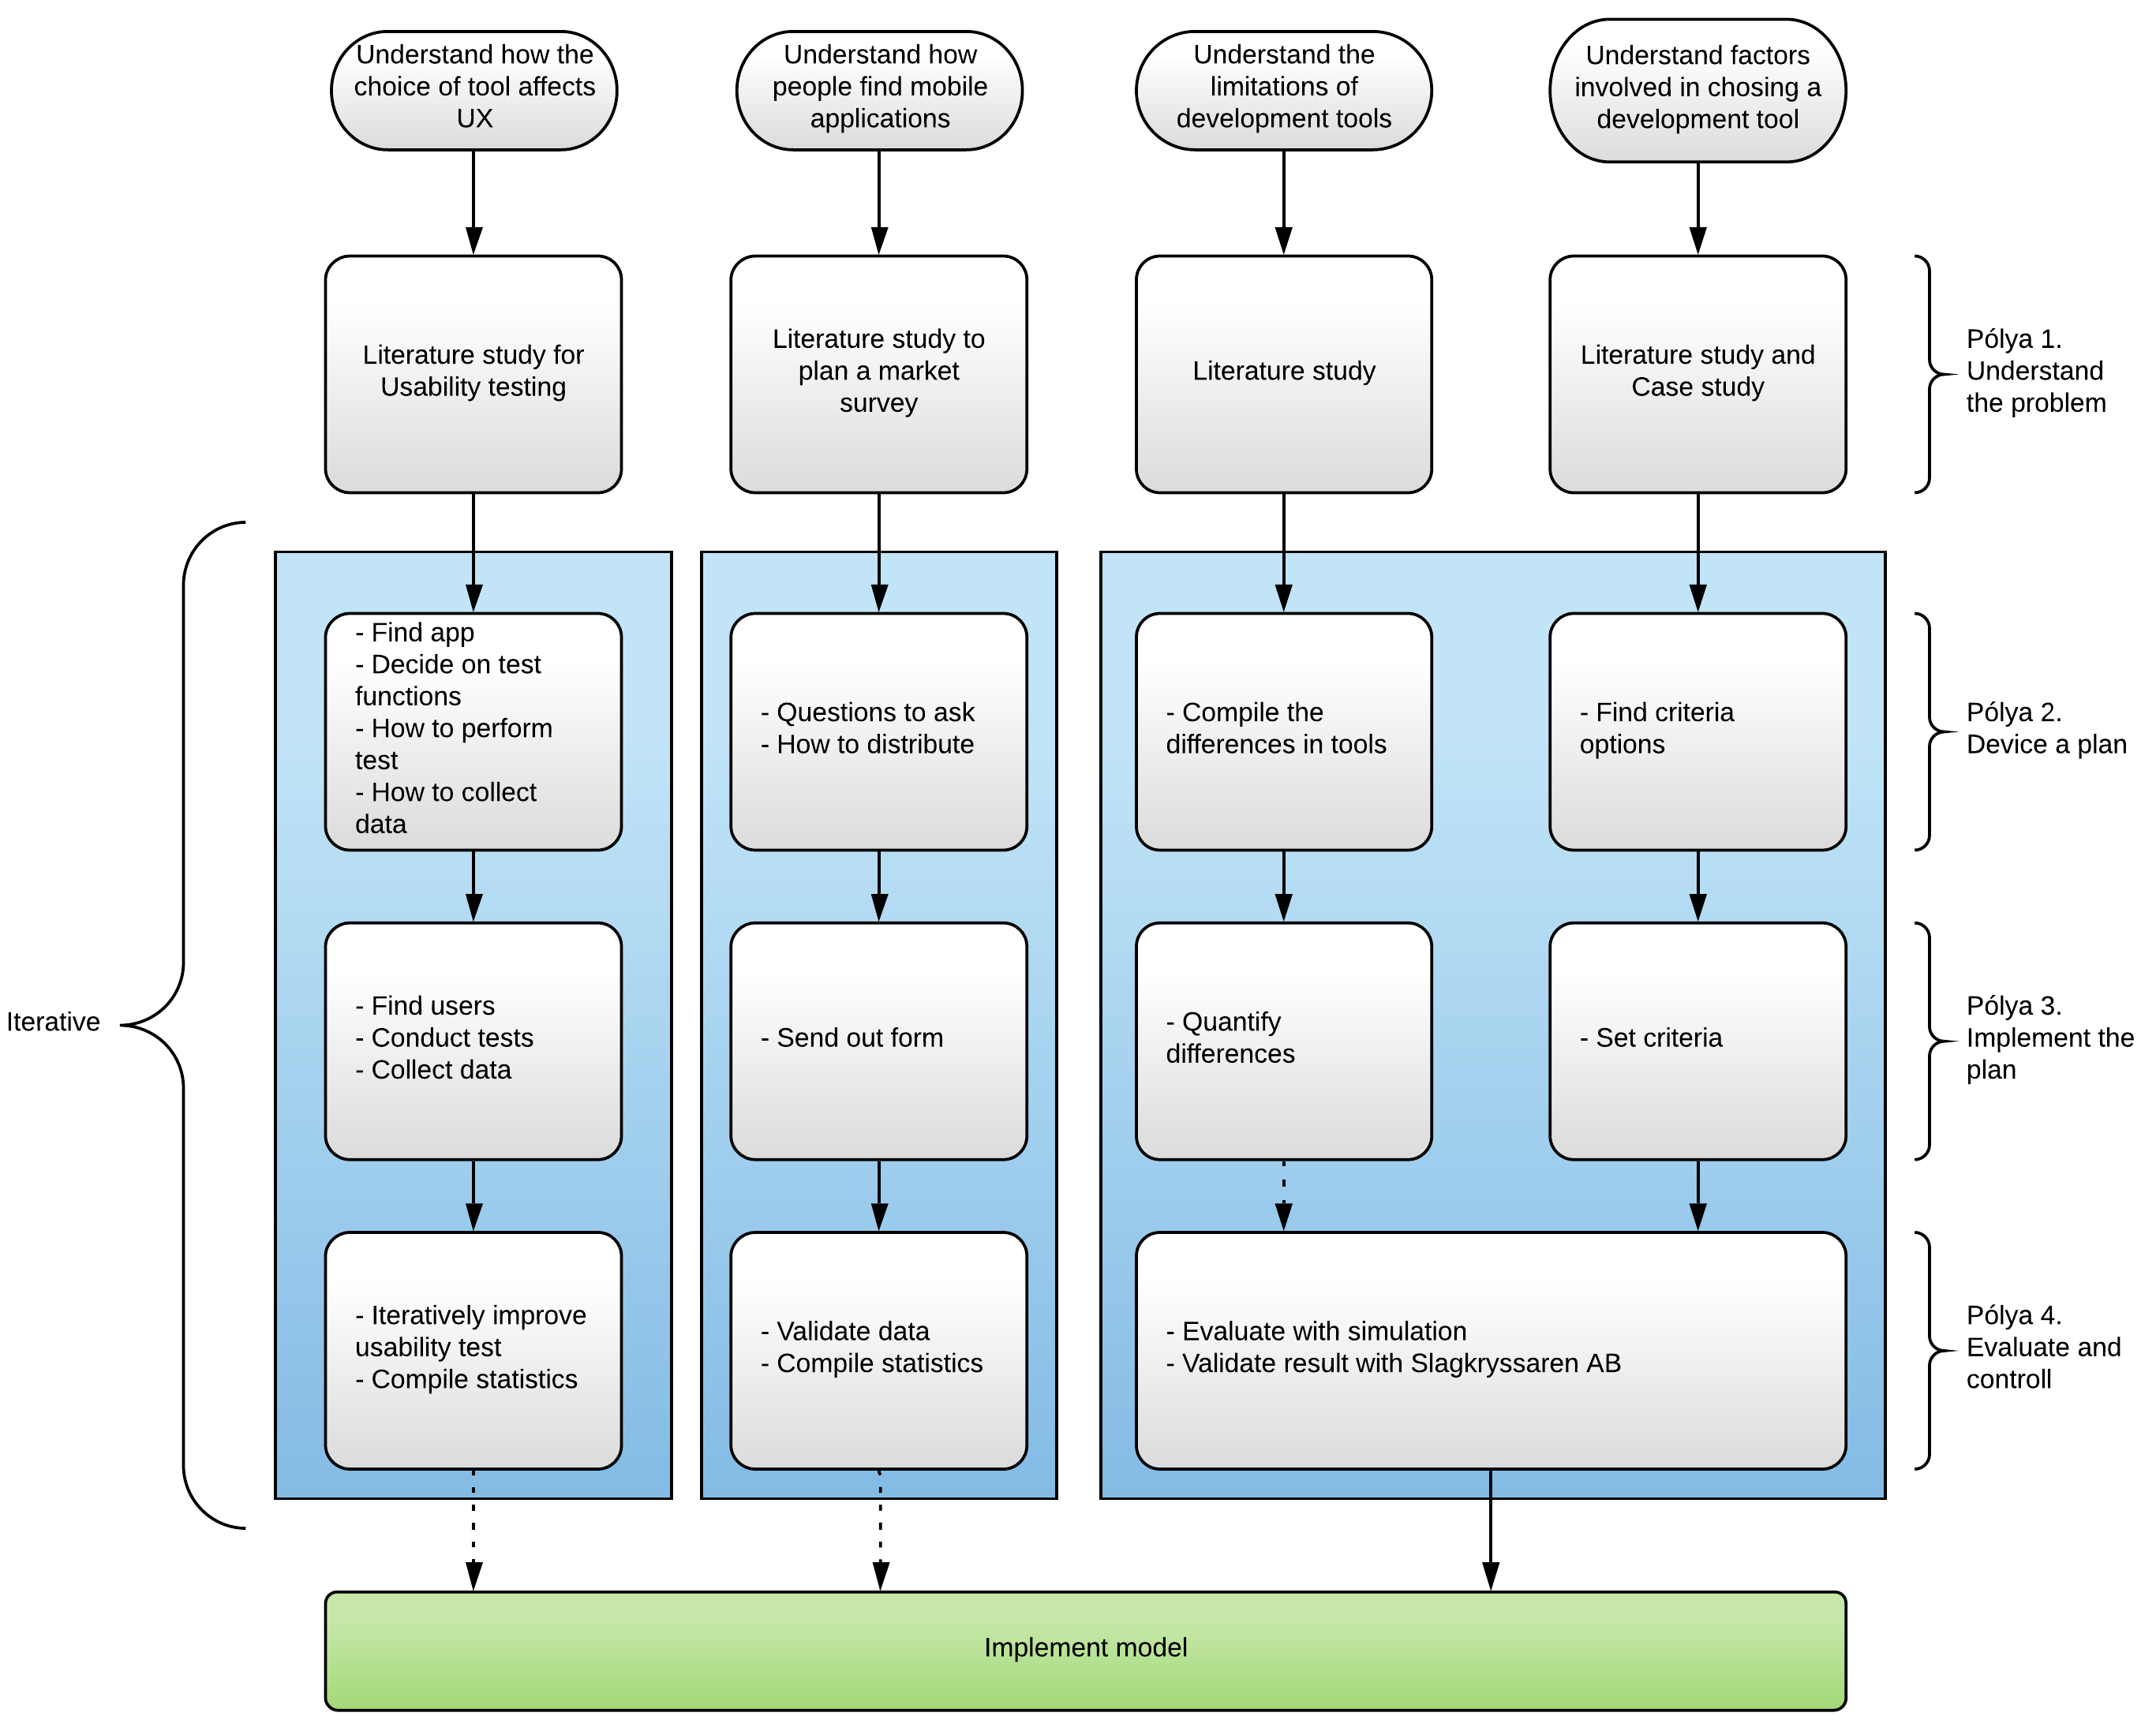
\includegraphics[width=1\textwidth]{img/polya2.png}
    \hfill
    \caption{\textit{Implementation of Pólya's four-step method.}}
        \label{fig:project-polya}
\end{figure}

\subsection{Project methodology}

The project methodology is a process which guides the project from a plan to a finished product. Resource management, cost efficiency and prioritization are some of the factors to consider when entering a new project, and following a well-defined project method would increase the chances of producing deliverable results with the resources available. 

\subsubsection{The project triangle}

The project triangle, shown in figure \ref{fig:project_triangle}, describes how the quality of the project correlates with the time, cost and scope  \cite{TheProjectTriangle}. The cost and time of this project were predetermined, so the only mobile variable was the scope. This means that the scope of the project could have been extended or cut as needed. This could have been applied to the usability tests, as more or fewer tests could have been conducted depending on the time left. Extending the scope could, for example, mean introducing more technologies into the model. The scope could also have been extended, improving the quality, if more tests had been conducted.

\begin{figure}[ht]
    \centering 
    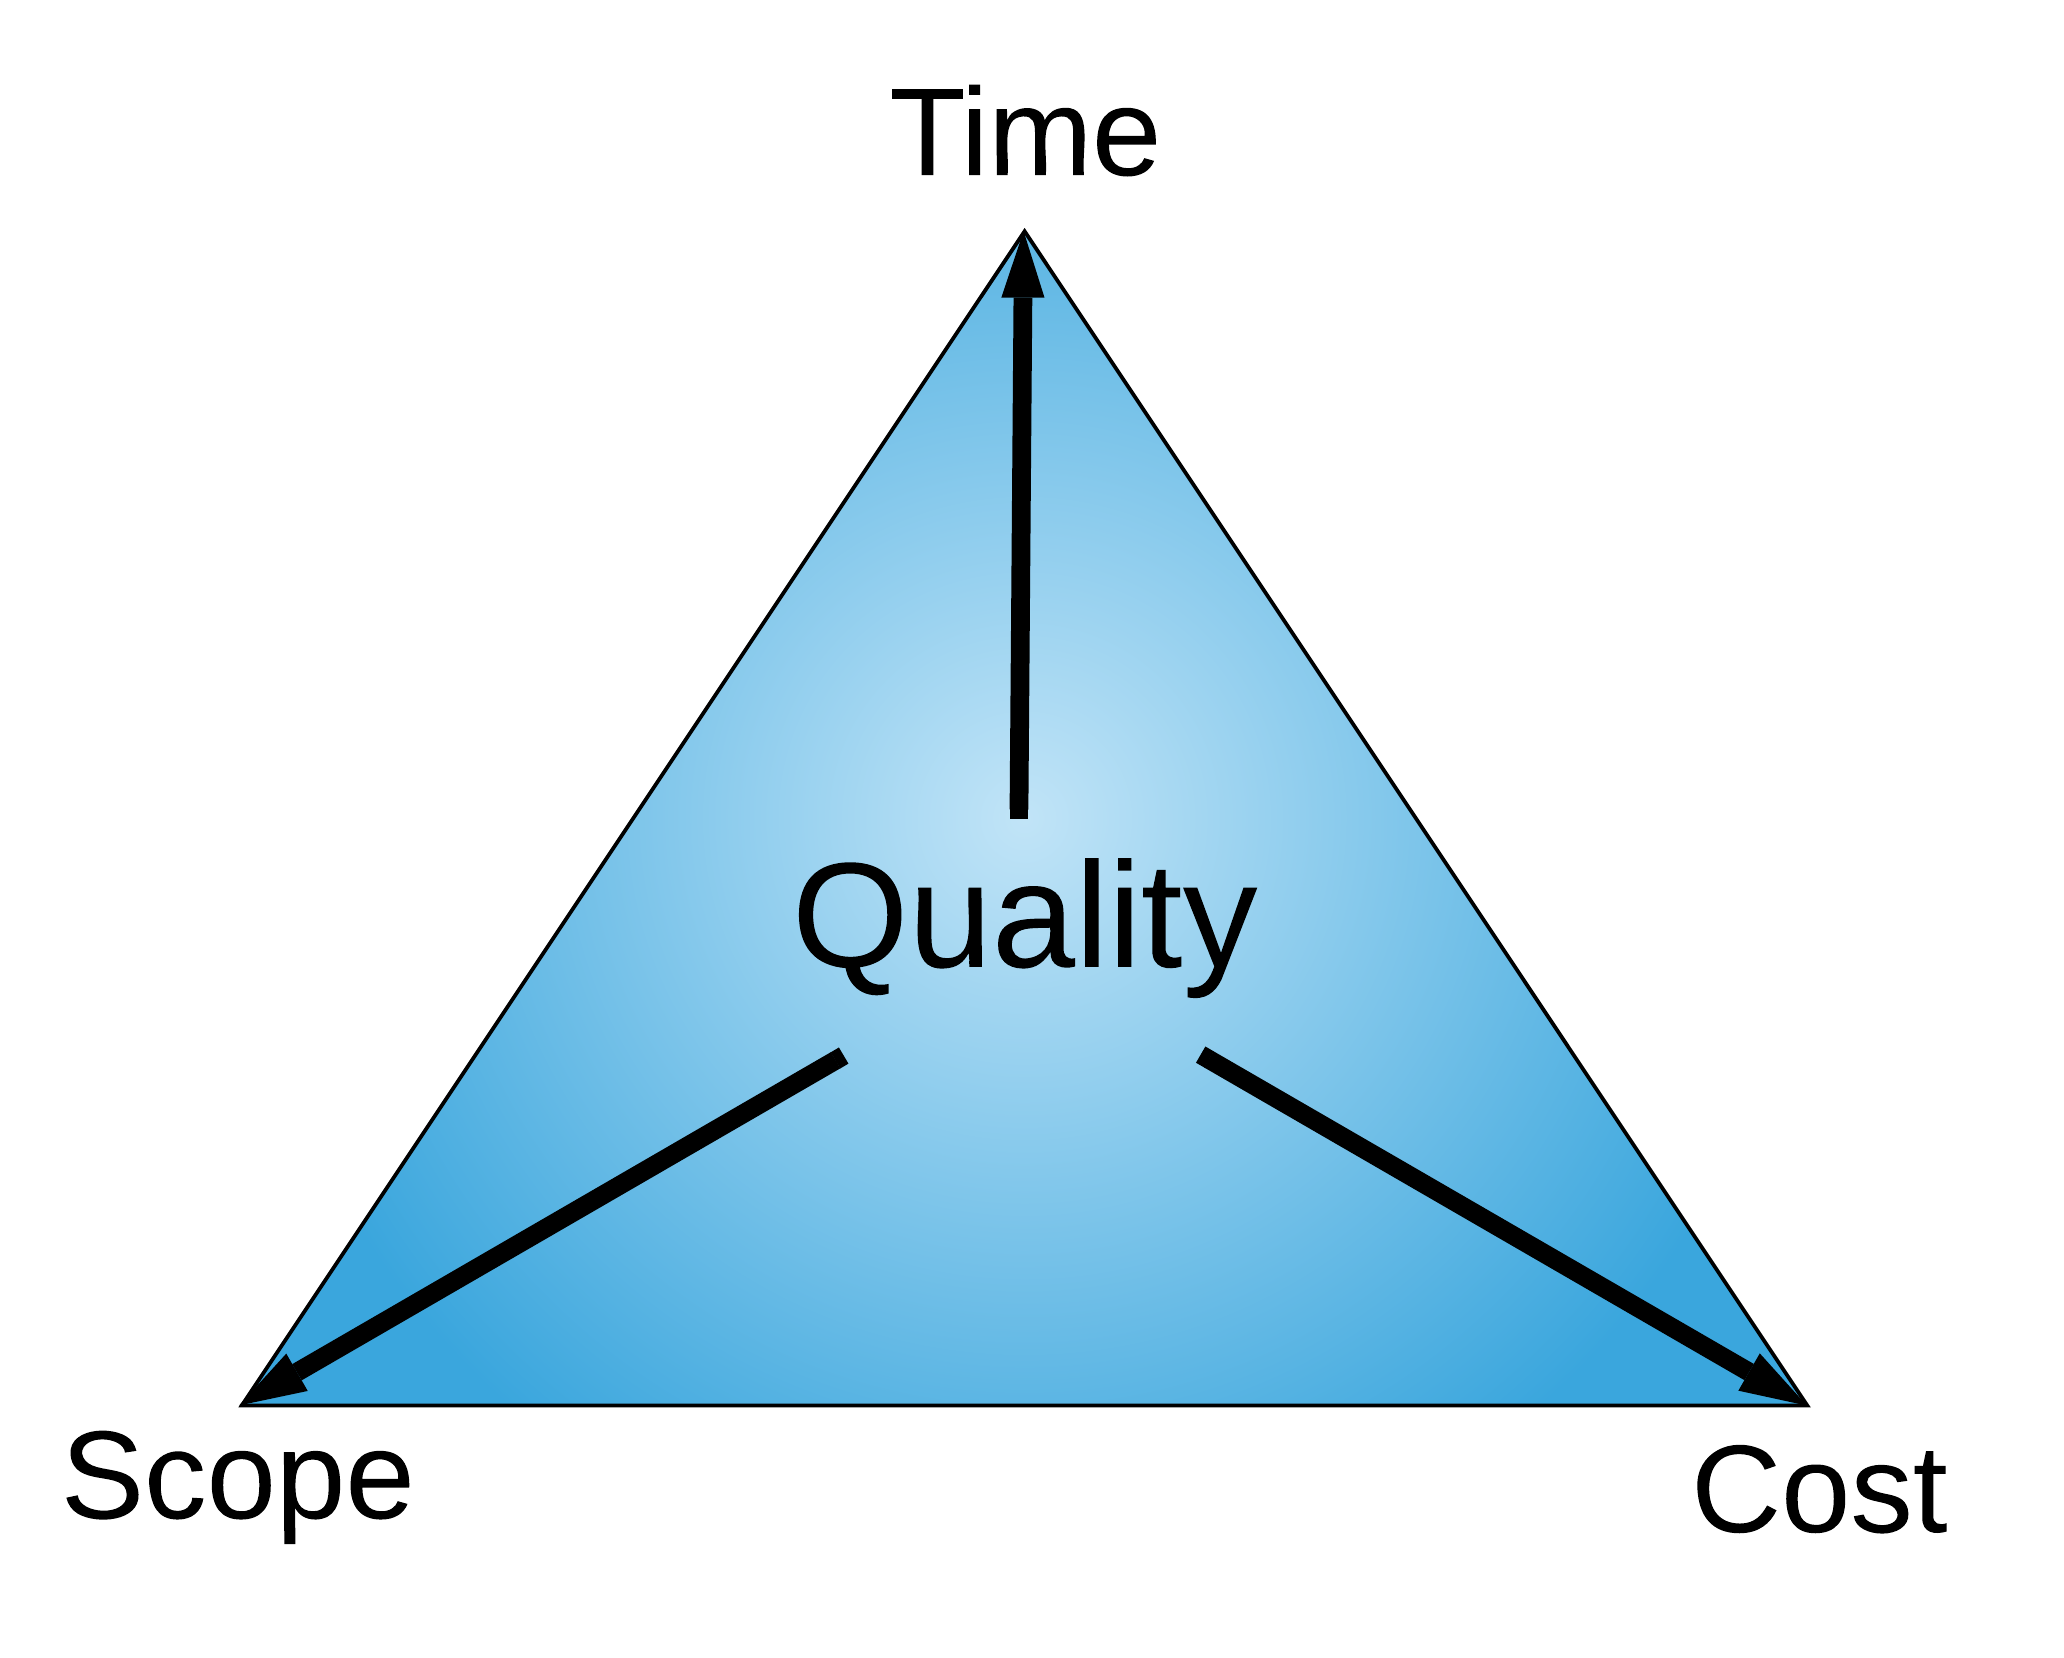
\includegraphics[width=0.6\textwidth]{img/project_triangle.png}
    \hfill
    \caption{\textit{The project triangle}}
    \label{fig:project_triangle}
\end{figure}

\subsubsection{MoSCoW}

MoSCoW is a method used to prioritize during project management \cite{MoSCoWforUX}. The term MoSCoW is an acronym for the four prioritization categories: Must have, Should have, Could have and Won’t have. The MoSCoW was chosen as a prioritization method for this project due to its ability to fraction the project into a core assignment and possible improvements. 
The MoSCoW for this project can be seen in figure  \ref{fig:MoSCoW}.

\begin{figure}[ht]
    \centering 
    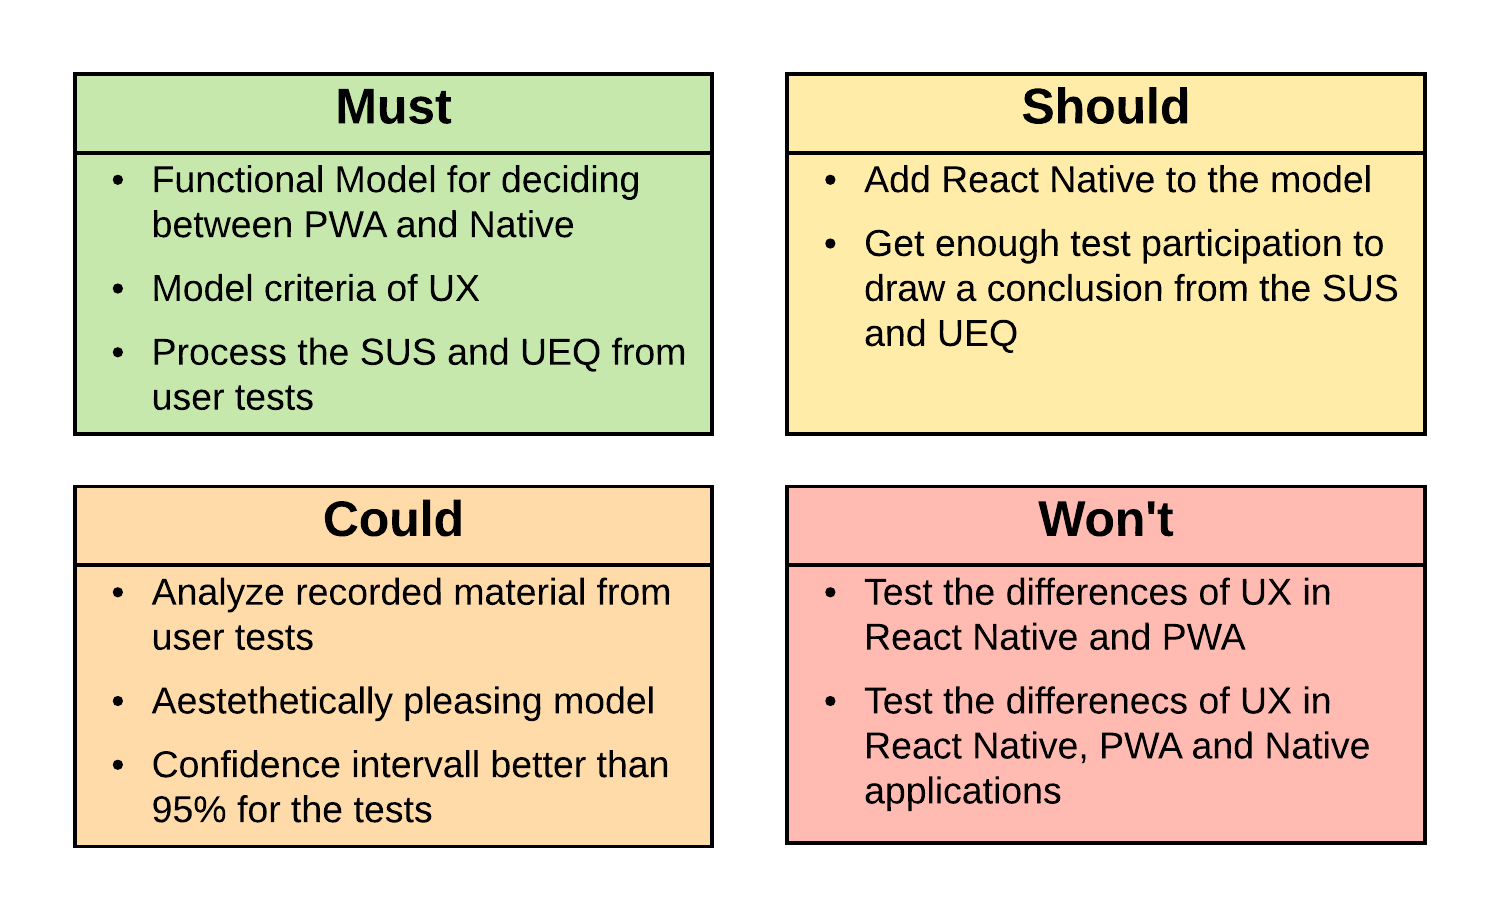
\includegraphics[width=0.9\textwidth]{img/moscow.png}
    \hfill
    \caption{\textit{MoSCoW chart of this project}}
    \label{fig:MoSCoW}
\end{figure}

\subsubsection{Connecting the dots}

With the research and project methodology explained and established it was easier to get hold of the overall picture of this study. The scope and iterations were limited by the time and the cost, two factors which this study could not affect. When the tasks of the MoSCoW category "Must" had been fulfilled, depending on how much time was left, more tasks from the categories "Should" and "Could" could have been added to the project.

\subsection{Literature Study}

To understand and explore the differences between the different types of mobile applications, extensive research had to be made. Mobile applications that use more of a hybrid approach, such as PWA or React Native, tend to follow trends. This means that if the technology does not get enough attention it might go extinct. This was at the time of writing happening to many JavaScript frameworks such as Angular, according to consultants at Slagkryssaren AB. The information available on this subject was both opinion- and research-based.

For the MCDM, the design practices and evaluation processes were investigated. 
To conduct usability testing, it was a requirement that these tests should follow typical practices currently in use. This includes how to design, conduct and validate usability tests.
Typical places where information was gathered were:

\begin{itemize}
    \item Blogs, forums and similar websites
    \item Research articles and technical literature 
    \item Opinions from developers and experts within interaction design
\end{itemize}

\subsection{Case study}

Since the model was to be used by Slagkryssaren AB, the development of the model was done in close co-operation with the company’s consultants. These consultants have extensive experience in the field of developing applications and choosing application development tools. This inductive approach was more suitable than a deductive one, as there was no decidedly right or wrong conclusion when choosing an application development tool.

Conduction of the case study was done by discussion with the consultants at Slagkryssaren AB. These discussion meetings were to be unstructured in an attempt to get richer, more qualitative data. A combination of planned and improvised discussions were held to answer questions emerging during the progression of the study. The meetings were held approximately once a week, and lasted around 40 minutes each.

\subsection{Mobile application discovery survey}

The survey was conducted to explore two hypotheses which emerged during the discussions with Slagkryssaren AB, one of them being that people tend to find information about applications mostly on the platforms application store, rather than using web searches. The other hypothesis was that Android users tend to look for information about applications through web searches, while iPhone users tend to go to the App Store first. This hypothesis was based mainly on the fact that smartphones running Android usually have a Google search bar pre-installed on the home screen. It would therefore be easier for them to just tap the search bar to find information, rather than opening the App store application which one has to do on iOS devices. These hypothesis were explored to understand the consequences of releasing an application which can not be found on the platform’s app store, which is the case for PWAs. 

\subsection{Usability testing}

To see the differences in user experience, usability tests were conducted. Usability testing was chosen as a method for measuring UX due to its relative simplicity and time efficiency.

During the tests, PWA and native applications had the main focus. React Native and PWA both use JavaScript but React Native can access native user interface components, meaning it is like a mixture of both types. To be able to perform the usability tests with all tree techniques we would have needed a similar application developed with all methods, something that was not available at that moment, and outside of the scope of this study to develop. 

To measure the differences in quality, usability, attractiveness and other UX-related criteria, validation of the tests was done using surveys. Several measuring methods for this exist, such as the System Usability Scale (SUS), the Usability Experience Questionnaire (UEQ), Net Promoter Score and the Standardized User Experience Percentile Rank Questionnaire. These surveys are popular for measuring how good the different applications are in certain criteria \cite{Rauschenberger2013, Kortum2014}. The surveys can only receive quantifiable data.  A better overview of the process of the tests is shown in figure \ref{fig:usability_test_process}.

The users tested two versions of the same application on the same platform they normally used. One of the application versions was a PWA and the other a native application.

The subject got a list of six tasks to perform on the application, and after using each version of the application the subjects filled in a UEQ and a SUS form. The results from these SUSs and UEQs formed the base for the quantitative data from the usability tests. During the tests, the moderator encouraged the subject to keep talking by asking questions about what the subject was doing. To fully understand the test subject’s experience, it was useful to have them think out loud. This means the subject says out loud what they are thinking and trying to do while testing the application, giving the researcher an insight into what the subject has troubles with and misunderstands in the product. Thinking out loud gave qualitative data from the users \cite{Nielsen2012}.

After both applications had been tested, the subject was asked more in-depth questions about their experience of the applications and their thoughts and feeling. This gave richer, more nuanced comparisons between the different applications, and qualitative information which could later be processed to further define how the criterion for UX should be scored in the model.

The recorded material from the tests was analyzed. The subjects’ feelings about the applications were interpreted through their spoken words, their facial expressions and verbal cues. This data was then quantified by processing the recorded material and transcriptions, in search of patterns in the subjects’ behaviour.

The results from the UEQ and SUS were plotted and compared between the two application. With this data, a confidence interval could be calculated and compared to the preferred confidence level. This result formed the basis for the criterion of UX.

\begin{figure}[ht]
    \centering 
    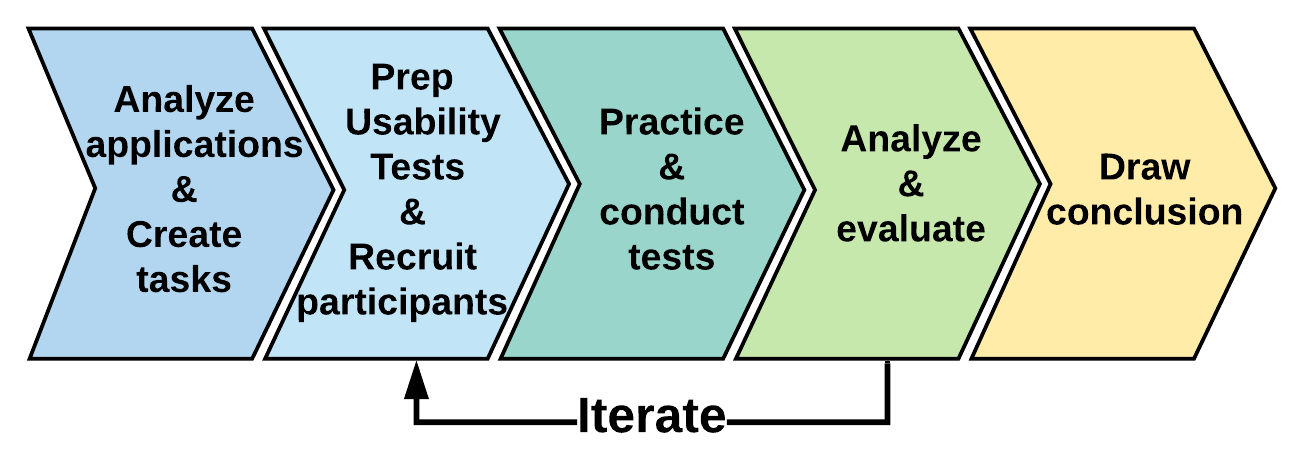
\includegraphics[width=0.9\textwidth]{img/usability_test_process.png}
    \hfill
    \caption{\textit{Process of performing a usability test}}
    \label{fig:usability_test_process}
\end{figure}

\subsection{Multi-Criteria Decision-Method}

To build a model which took usability into account, the comparative usability test was conducted. This inductive approach would produce qualitative data. The different solutions tested in a comparative usability test could be tested either separately on the different test subject, or together on the same subjects. In this study, both solutions were tested on all test subjects. A drawback with this method is that there could emerge a pattern that the user would like a particular version if they are tested in the same order \cite{Ross2017}. To counteract this effect the subjects tested the applications in varying order so that the bias would have the same impact in both directions, hopefully cancelling out in the end. This was done since the scope of the study was comparatively small, meaning the benefit of more test subjects was vital.

To make the results as comparable as possible, we chose to have all the test subjects perform the same set of tasks. The tests were conducted on the same OS that the test subject normally used, to minimize confusion due to an unknown platform  \cite{Schultz2006}. 
For the model, it was also relevant to include application exploration as a criterion. To acquire quantitative data for the finding and downloading habits of the population, a cross-sectional survey was conducted. This gave data from a more diverse population than is possible from qualitative methods, such as interviews, in the span of the study. 

The model itself was based on the MCDM method. The MCDM uses a mathematical function to calculate the best alternative when faced with a decision involving many different criteria. The decision-makers decide which criteria are important and rank them. The possible alternatives are then scored on each criterion. The alternative with the highest score is then the best alternative for that decision-makers ranking.

Several MCDM methods could have been applied to this study. WSM was chosen due to its simplicity of calculation. Since the WSM demands the data to be quantifiable, all qualitative data gathered was translated into quantitative data. 
Mobile application discovery was researched with an online survey, producing quantified data. 

For the tests, quantification was done with surveys and questionnaires where test subjects quantified their own experience with the application, in combination with analyzed facial expressions and behaviour from the recordings.

The criteria were based on input from results of our test and survey, scientific articles, software development websites and discussions with consultants at Slagkryssaren AB.

When a set of criteria was decided, scores were given to each alternative development tool in the model. The scores were set based on previous literature study. These scores were presented to the consultants at Slagkryssaren AB and were iteratively improved upon based on their feedback.

When scores were set for the alternatives, the next iterative phase began. 
Use cases were run through the model, and the result was assessed. If the outcome was seen as unreasonable or unlikely to be chosen, the scores and criteria were reassessed. This iterative process was to be repeated until reasonable results are acquired, or until there was no more time to reiterate. 

\subsection{Technical method}

In order for this study to be carried out, there was need to include some tools. Testing different ways of calculating the decision-making model and analyzing the data from the survey, UEQ and SUS was done using \textit{Google sheets}. Gathering the data for the tests and survey was done using \textit{Google forms}. The recording of the usability tests was done using an \textit{Asus} laptop and a \textit{GoPro Hero 4 Session}. All the gathered data and other media were stored on \textit{Google drive}. The devices that were used for the tests are \textit{Apple iPhone 11 Pro} and \textit{Oneplus 5}. The model was implemented using the javascript framework  \textit{Vue.js}, and stored on \textit{GitHub}.  
\section{<The Work> }
Describe the degree project. What did you actually do? This is the practical description of how the method was applied.

\section{<Result> }
Describe the results of the degree project.

\section{ Discussions }

This chapter presents the research questions and methodically goes through how well they were answered. After this, a discussion on how each part of the project could have been done differently to improve the accuracy of the results takes part. 

\subsection{Discussion}

The scope of this project was the only non-constant variable for affecting the quality. To get useful results from the usability tests, it was planned to perform 20 tests at least. Only 18 tests were conducted, as it was harder to find test subjects than we thought, and also to have time to properly analyze the material from the tests and implement the model. However, after 18 tests were conducted, the time planned for the usability tests was up. It was apparent that some parts of the data would not be improved with just a few more tests, but would require a much larger study. 

\subsubsection{Mobile application discovery survey}

As presented in Chapter \ref{section:research_methodology} the task of finding mobile applications was answered using a survey. The mobile application discovery survey was filled in by 94 persons. The ages ranged between 20 and 73, a more realistic outcome of the survey could probably be reached if it had included those below 20 as well. The survey was distributed in social media only, limiting the reach of the participants. A survey spread through other types of media as well would increase the scope and improve the results. 

After the survey was conducted, the following questions were found to be poorly worded:

\begin{itemize}
    \item \textit{"You just heard about a new smartphone application (app). Where do you turn when you want to find information about the app?"}
    \item \textit{"You just heard about a new smartphone application (app). Where do you turn when you want to download the app?"}
\end{itemize}

A better formulation would have been as follows:

\begin{itemize}
    \item \textit{"You are searching for new smartphone applications (apps). Where do you turn when you want to find information about the apps?"} 
    \item \textit{"You are searching for new smartphone applications (apps). Where do you turn when you want to download the apps?"}.
\end{itemize}

This might have improved the accuracy of the survey as the desired statistics was on how people find \textit{new} applications, and the way the questions were asked it could be interpreted as the question being about known applications. 

For the data collected to be useful in any statistical context it would have required that some more information on the participants was collected. It would be useful to know how knowledgeable the subject is on new technology, how much the subject uses their smartphone, level of education and occupation. Knowing this, one could compensate for a skewered participant population compared to the general population.

\subsubsection{Usability test}

As presented in Chapter \ref{section:research_methodology} the task of UX was investigated through usability testing.
The results of the usability tests suggest that there was a difference in how a user perceives a PWA and a native application, and that overall the native application was preferred. Two out of the five included aspects of the usability test UEQ had results which were statistically significant, even on the relatively small amount of participants used in this survey, indicating that the difference is substantial enough to affect the users experience of the application. 

The usability tests were conducted during office hours, and the participants were recruited through university campus channels. This resulted in the participants almost exclusively being students at a technological institute. The tests were conducted in Slagkryssaren ABs office in the beginning but were later moved to the campus of the university. This was done to ease the process of recruitment, as holding the tests in the office resulted in added travelling time for the student participants. It also opened up for the possibility of having drop-in times for participating, instead of having to book a time in advance.

The age range was also limited to young adults between 20 and 30 years old. This means the participants were likely more experienced and comfortable using new mobile software than the average person. An improved result could have been achieved if there was a wider demographics of participants, which would demand that the tests be performed outside of office hours and in several different locations. Recruitment could have been performed on several different platforms, targeting harder-to-reach demographics. The participants were compensated for their time in a goodie-bag consisting of candy. Monetary compensation could have attracted more participants, but there were no funds for such compensations in this study.

There were some technical limitations to the usability test. The iOS device used was a relatively new iPhone 11 Pro, whereas the Android device was an older OnePlus 5. There were no newer Android devices available to test on, so the iPhone used for the tests had noticeably better performance than the Android device. Due to the low performance of the Android device, it was possible the PWA was given a disadvantage compared to how it would perform in real life on most users' personal devices. This did, however, give a good insight into how a PWA might perform on a lower-end or older device.  An ideal scenario would have been to use one newer and one older device from each platform, with comparable performance.

There were also some technical difficulties to take into consideration. During one of the tests, the WiFi-connection was down, forcing the moderator to intervene which might have affected the test subject's impression of the PWA negatively. A stable, monitored internet connection would have prevented these problems. For a few of the tests, some parts were not captured on camera from behind, meaning the device's screen was not shown. This was due to the difficulty in recording and charging the camera simultaneously, resulting in the camera running out of battery.

Since the test conductors were each responsible for one of the two platforms, one person got to practice moderating and the other recording more. This affected the quality of the written material and the instruction-giving for the test subjects. This could have been avoided if the same person had been moderator or recorder for every test, but since the conductors were not experienced with the other device this was not optimal for this test. Screen recording and eye-tracking technology could have eliminated the need for a recorder, which would improve the accuracy of the material. With recorded material mainly in the form of notes made by a human, there is always the risk of a bias towards one of the products. With the limited time frame and finances of this study, it was not possible to gather and process the amount of material that would be produced by implementing these technical solutions.

Due to time limitations, the recorded material could not be processed in detail. Instead, the written material compiled at the tests was used as a base for the qualitative data, and when there were uncertainties in the written material the video recordings were reviewed for clarity.

The test conductors had limited experience in the field of Human-computer interaction. There is a risk that useful material from the usability tests was overlooked or misinterpreted due to lack of experience. 

\subsubsection{Decision model}

As presented in Chapter \ref{section:research_methodology} the tasks deriving from the research question of implementing a model were investigated through conducting literature and case studies. That information would then be used for the process of designing, implementing and evaluating the model.
The decision model was implemented with WSM. It is possible a version of AHP would have produced different results, as it would force a more polarizing opinion from the decision-maker. For an AHP implementation, the criteria would have to be re-evaluated, as the complexity of the AHP increases with every new criterion added. 

Some studies on the performance aspect of PWAs exist, but it was hard to decide on a clear number of how good or bad it was compared to native applications. The performance of an application, regardless of the development method, is highly dependent on how the application is coded. A well-coded PWA could perform better than a native application with poor implementation. For the model used in this study, what would be considered a well-implemented native application was taken into consideration when setting scores and compared to a well-implemented PWA. How well this model translates to real life was uncertain, as trying to compare how well applications are implemented was a very complex task.

The Budget criterion was highly simplified. Many factors not included in the model could affect the economical aspects of choosing a development method, including the revenue model of the business and the effect of improved search engine optimization.

Overall it was difficult to quantify the scores for the model. This resulted in the scores being set partly on a trial-and-error basis. A possible solution to this would have been to use a Knowledge-Based System (KBS) to build the model. A KBS uses artificial intelligence to predict which solution is most advantageous, comparing an input to the input from several other solved scenarios. This could give a solution which is correct with a certain probability, which would increase when more scenarios are run through the model and evaluated. The KBS bypasses the need for quantification, eliminating the risk of a faulty score affecting the outcome of the model \cite{Brent1986}.

The decision model for React Native specifically was limited by the complexity of the available functions. React Native can behave similarly to a native application if implemented with the proper wrappers, but different functions have different limitations and opportunities. We decided to instead just raise the score on Functions to a level agreed on by the developers at Slagkryssaren AB to be an appropriate approximation of a React Native applications functionality.

\section{Conclusions}


In this chapter, the final conclusions on the projects findings are presented. Finally, in the section Future Work, research which could be conducted in the future on the topic of this project is discussed. 

\subsection{Conclusion}

\textit{Do users notice a difference between progressive web applications and native apps, and does the difference affect the user experience?}

According to our findings yes, to a certain extent. The biggest difference between PWAs and native applications was at the time of writing the limitations on functions available, but even when functionality is not taken into consideration we would still argue that PWA was shown to be worse from an end-users perspective. We say this because the difference between the native application and PWA was significantly noticeable when it came to response time, at least on the older device tested. It was possible we could have gotten a different result if we had tested with a different application. When trying to find an application to perform the tests on, another product called Pinterest was considered. However, the PWA for Pinterest did not work on the iOS device available so it was not selected for this test. The PWA on Pinterest was more similar to the native application and would otherwise have been a good choice for the tests. Our conclusion from the usability tests is that when the device running the application has outdated hardware the PWA would not perform as well as a native application. However, it was also possible that the PWA for Yummly was simply not as well-implemented as its native counterpart.

Something to take into account is that from the survey we noticed that half or more of users will probably try to find the application through the phones app store first. If this was a trend among the population in general this could mean that users would need to do more searching in order to find the PWA than a native application. There also seems to be a trend that iPhone users primarily find information about applications through app store. However, this was not a big enough survey to convey a definite conclusion on the matter. 

\textit{Can a model accurately decide whether a PWA, a React Native application or a native application is most favourable?}

Yes and no. After presenting the model to Slagkryssaren AB the consultants expressed the opinion that the model seemed to give accurate results based on the input given. The recommendation from the model in itself was not a definite truth, but the recommendation in combination with process of filling in the form gives a good ground for discussion. This could be helpful to challenge a fixed idea of what application to implement, either within the development team or when discussing with a customer.

The subject of choosing a development tool is subjective in its nature, it was therefore not unexpected that the model would be used more as a tool for discussion and prioritization than a definite decision-making tool.

\subsection{Future Work}

A usability test including PWAs, native applications and hybrid applications such as React Native could further improve the reliability of a decision model, as the UX criteria for React Native in this model was based entirely on opinion from developers at Slagkryssaren AB.

The score for the criteria Maintenance was also based on opinions from developers. An improvement would, therefore, include basing this number on some kind of statistics, analyzing how much more maintenance a PWA needs compared to other applications. For the Budget criterion to be more precise, research on how the revenue is affected by where an application is downloaded and which payment methods the end-users can utilize is necessary.

A larger study on application exploration could also be enlightening in the choice of application development technique. It would be useful to compare how different demographics find new applications, to find out the true impact of an application being present or absent on the most popular app stores.


% \include{content}

\newpage
\addcontentsline{toc}{section}{References}
%\textbf{If you are using mendeley to manage references, you might have to export them manually in the end as the automatic ways removes the "date accessed" field}
\printbibliography

\newpage
\section*{Appendices}
\appendix
\newpage
\etocdepthtag.toc{mtappendix}
\etocsettagdepth{mtchapter}{none}
\etocsettagdepth{mtappendix}{subsection}
\etoctocstyle{1}{Appendix - Contents}
\tableofcontents
\newpage


\section{Consent forms}
\label{appendix:consent_forms}
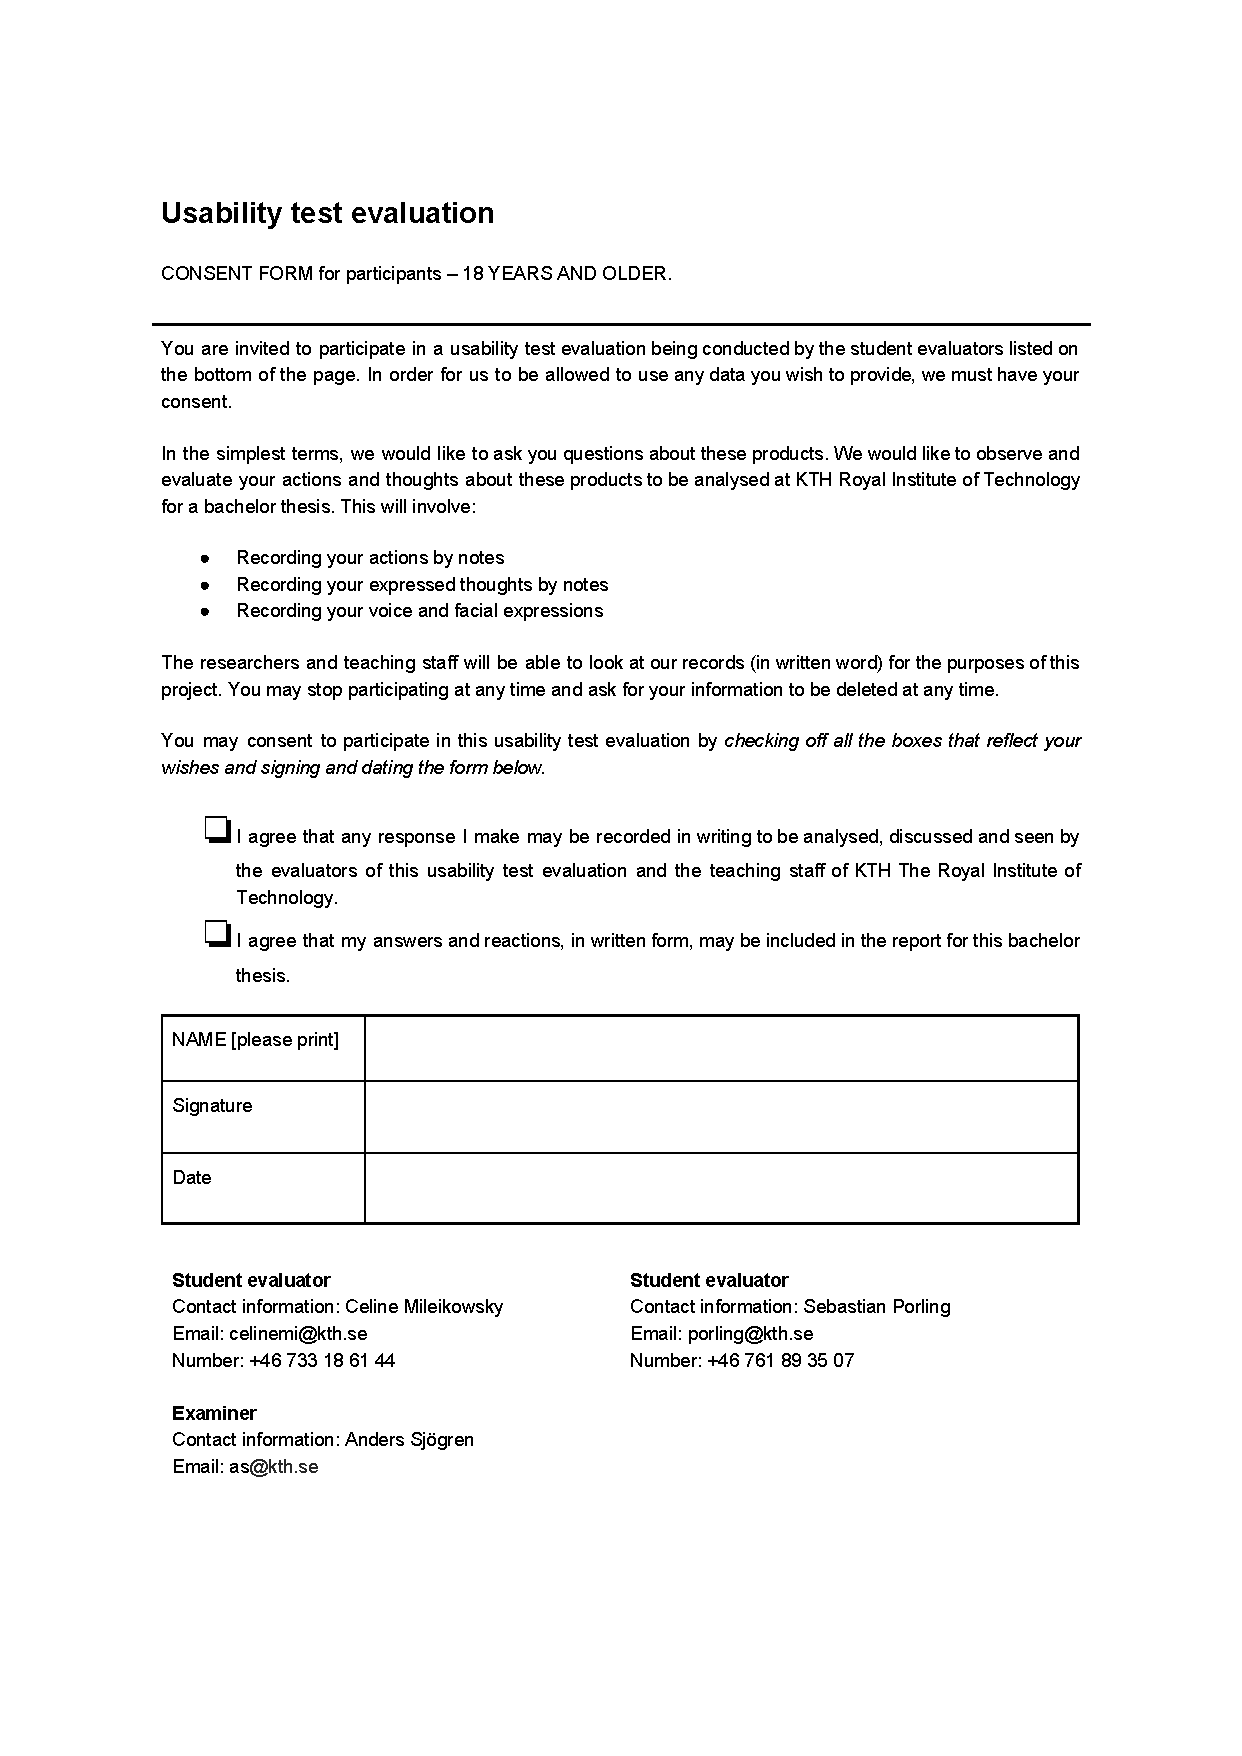
\includepdf[page={1}]{appendices/Consent_form.pdf}
\includepdf[page={1}]{appendices/Samtyckesformulär.pdf}

\section{SUS Data}
\label{appendix:a}
\begin{figure}[ht]
	\centering 
    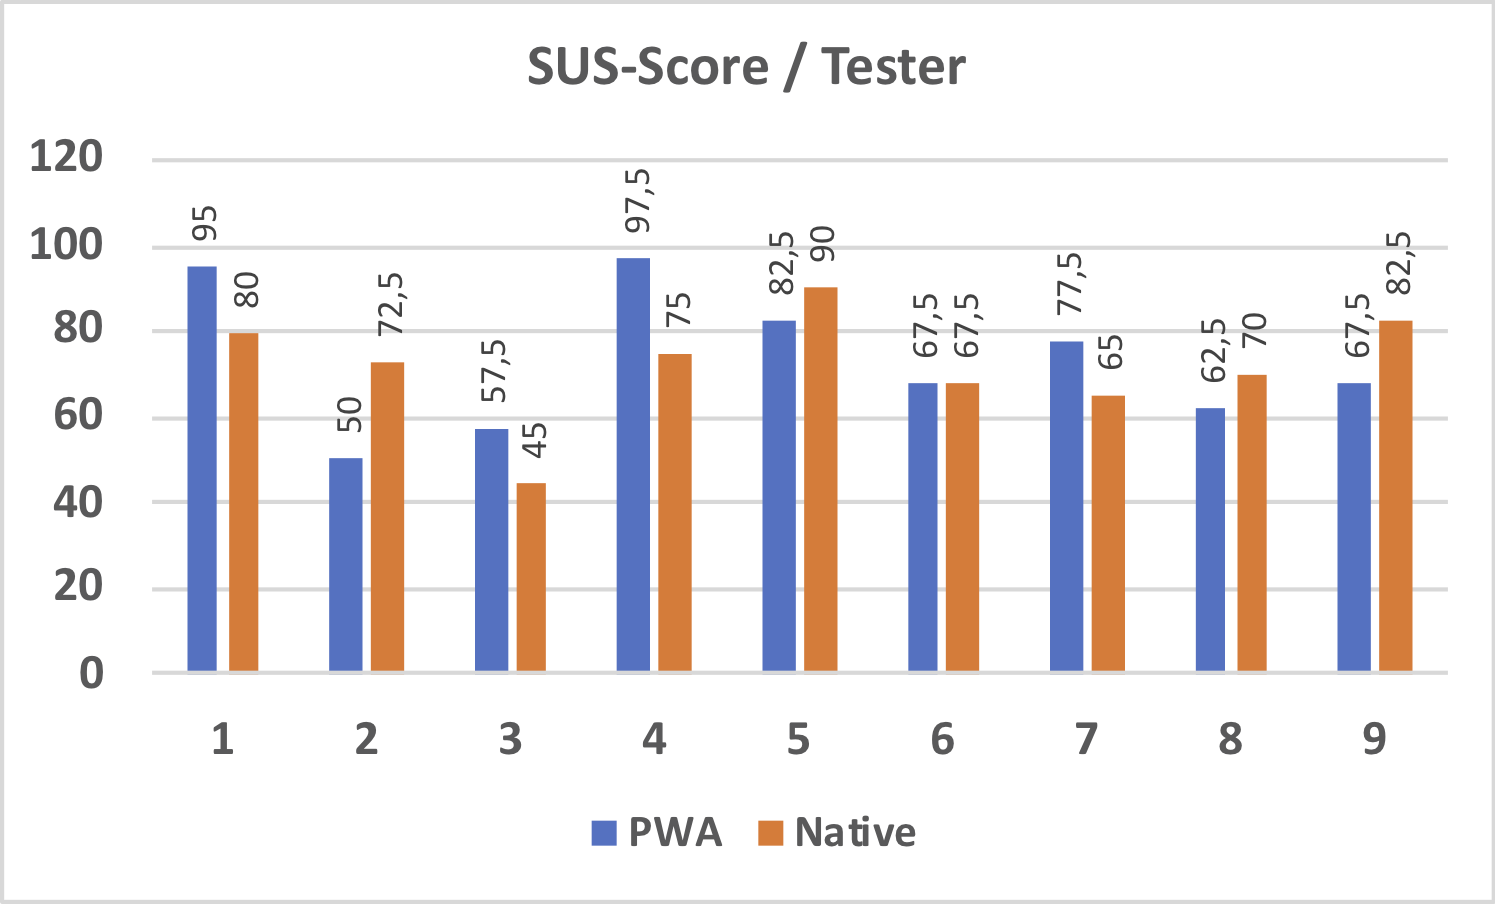
\includegraphics[width=0.8\textwidth]{img/SUS-Score_Bilaga1.png}
	\hfill
	\caption{\label{fig:SUS-Result1}{SUS results from Usability Test}}
\end{figure}
\begin{figure}[ht]
	\centering 
    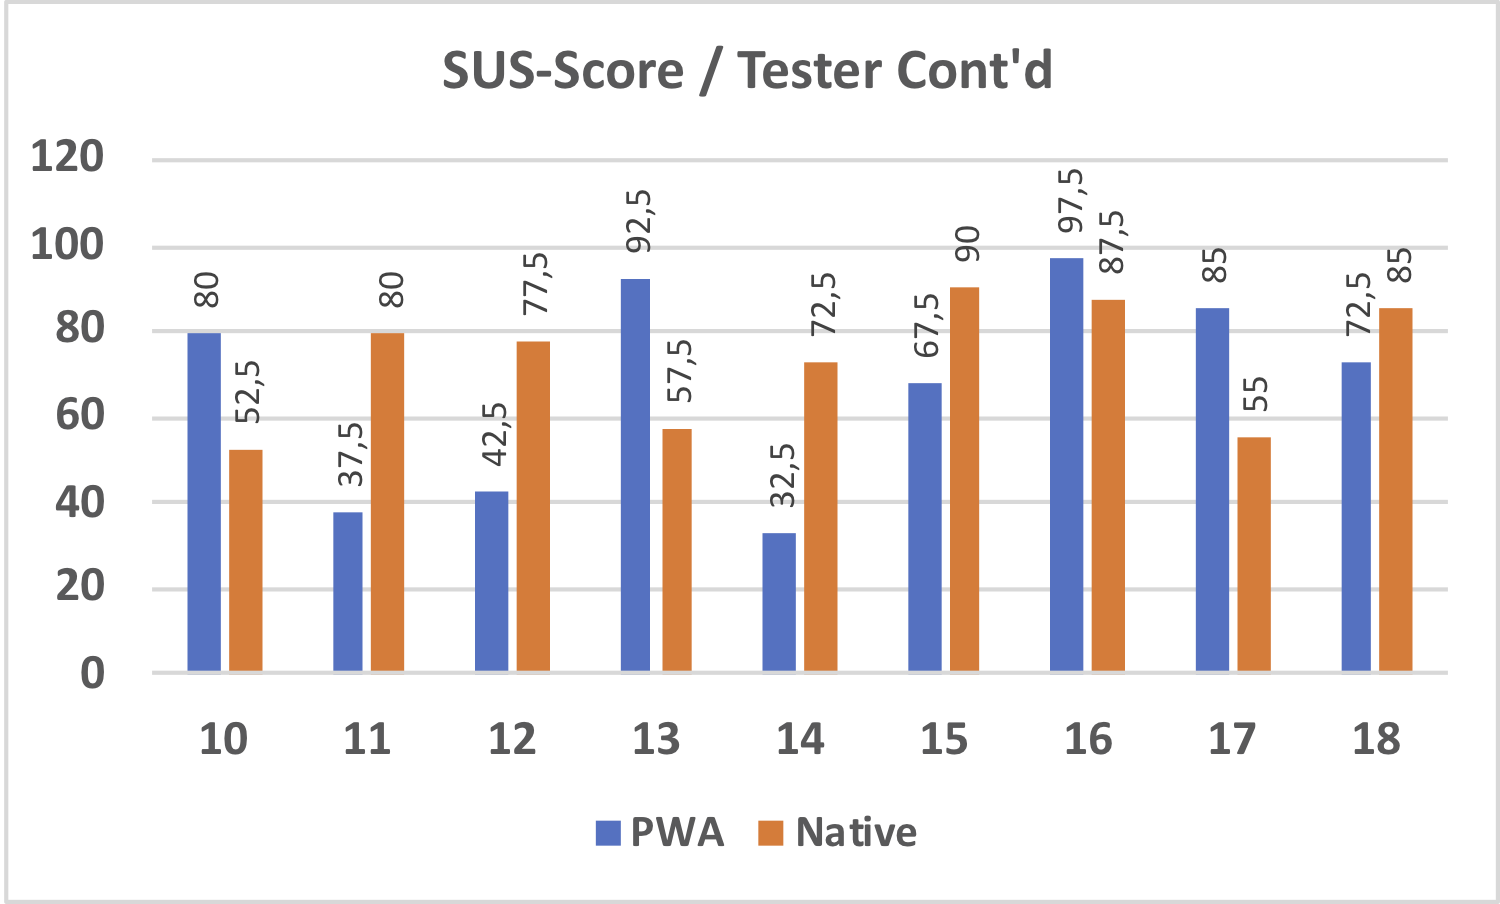
\includegraphics[width=0.8\textwidth]{img/SUS-Score_Bilaga2.png}
	\hfill
	\caption{\label{fig:SUS-Result2}{SUS results from Usability Test}}
\end{figure}
\newpage

\section{Survey Data}
\label{appendix:b}
\begin{figure}[ht]
	\centering 
    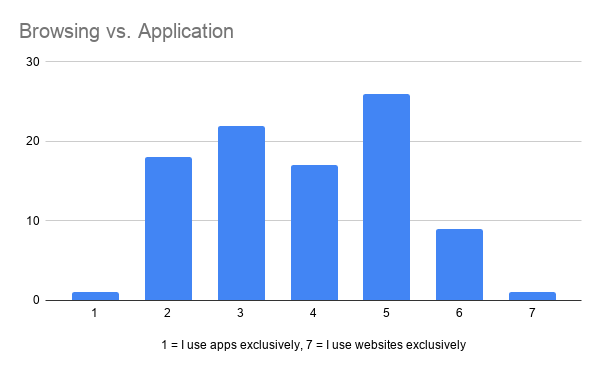
\includegraphics[width=0.8\textwidth]{img/Browsing_vs_Application_survey.png}
	\hfill
	\caption{\label{fig:Browser_application_data}{Survey results for the browsing vs applications question.}}
\end{figure}
\begin{figure}[ht]
	\centering 
    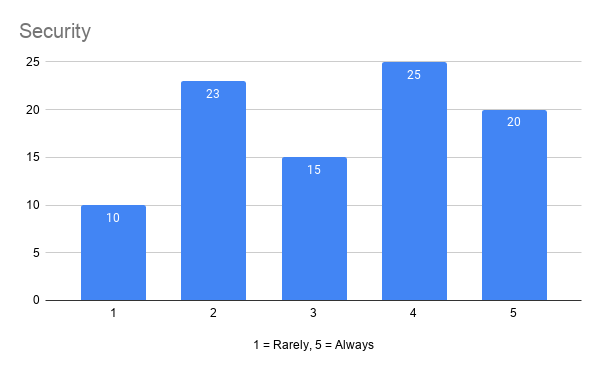
\includegraphics[width=0.8\textwidth]{img/Security_survey.png}
	\hfill
	\caption{\label{fig:Security_data}{Survey results for the question regarding security.}}
\end{figure}
\begin{table}[ht]
    \centering
    \begin{tabular}{ |>{\columncolor{light-gray}}c|c|c| } 
        \hline
        \rowcolor{light-gray}
        c = 0,05    & App vs. Browser usage  &   Security\\
        \hline
        Mean    &   -0,148  &   0,234 \\ 
        \hline
        Std     &   1,359   &   1,323\\ 
        \hline
        Confidence  & 0,274   &   0,267 \\ 
        \hline
    \end{tabular}
    \caption{\label{tab:total-survey}The result from survey in regards of application usage and security awareness.}
\end{table}


\newpage
% This is the last page of the document
\thispagestyle{empty}
\AddToShipoutPictureBG*{%]
    \AtPageLowerLeft{%
        
\includegraphics[width=1.0\paperwidth]{img/kth-footer}%
    }%
}

\PlaceText{20mm}{282mm}{\color{white}\fontsize{12}{0}\sffamily www.kth.se }


\end{document}
